%!TEX root = ../main.tex
%---------------------------------------------------------------------------------------------------
\FloatBarrier\section{Structural models for policy-making}\label{Framework}
%---------------------------------------------------------------------------------------------------
In the following section, we discuss uncertainty propagation and the common practice of using estimated parameters as a plug-in replacement for the true model parameters. We then explore the limitations of this strategy and introduce our alternative approach, in which we implement estimated confidence sets to construct uncertainty sets. In so doing, we are able to cope with uncertain policy predictions in a proper decision-theoretic framework. \\

\noindent At a high level, a structural microeconometric model provides a mapping $\M(\btheta)$ between the $l$ model parameters $\btheta \in \bTheta$ and a quantity $y$ that is of interest to policy-makers.
%
\begin{align*}
  \mathbb{R}^l \supset \bTheta \ni \btheta \mapsto  \M(\btheta) = y
\end{align*}
%
\noindent A policy $g \in \G$ changes the mapping to $\M_g(\btheta)$ and produces a counterfactual $y_g$.\\

\noindent Estimation of a baseline model $\M(\btheta)$ describing the status-quo on observed data allows researchers to learn about the true parameters. Frequentist estimation procedures such as maximum likelihood estimation and the method of simulated moments produce a point estimate $\hat{\btheta}$. However, uncertainty about the true parameters remains.\\

\noindent Previewing our empirical analysis of \citet{Keane.1997}, our $\M$ is provided by a dynamic model of human capital accumulation, which we estimate on observed schooling and labor market decisions using simulated maximum likelihood estimation. The policy $g$ is the implementation of a college tuition subsidy, and the counterfactual is the level of completed schooling in the population. Example parameters that drive the economics of the model are time preferences of individuals, the return to schooling, and the transferability of work experience across occupations.\\

\noindent The following illustrative example highlights our key points. We consider two policies $g \in\{1, 2\}$  that result in two different mappings $ (\M_1, \M_2)$ of the same scalar $\theta$ to a counterfactual $y_g$. Higher values of $y_g$ are more desirable for a policy-maker. The point estimate $\hat{\theta}$ is determined by estimating a baseline model on an observed dataset. We denote the probability density function of its sampling distribution by $f_{\hat{\theta}}$.\\

\noindent Under the first policy, the counterfactual is an increasing nonlinear function of $\theta$. In the case of the second policy, the relationship is decreasing and linear.
%
\begin{figure}[ht!]\centering
\scalebox{0.35}{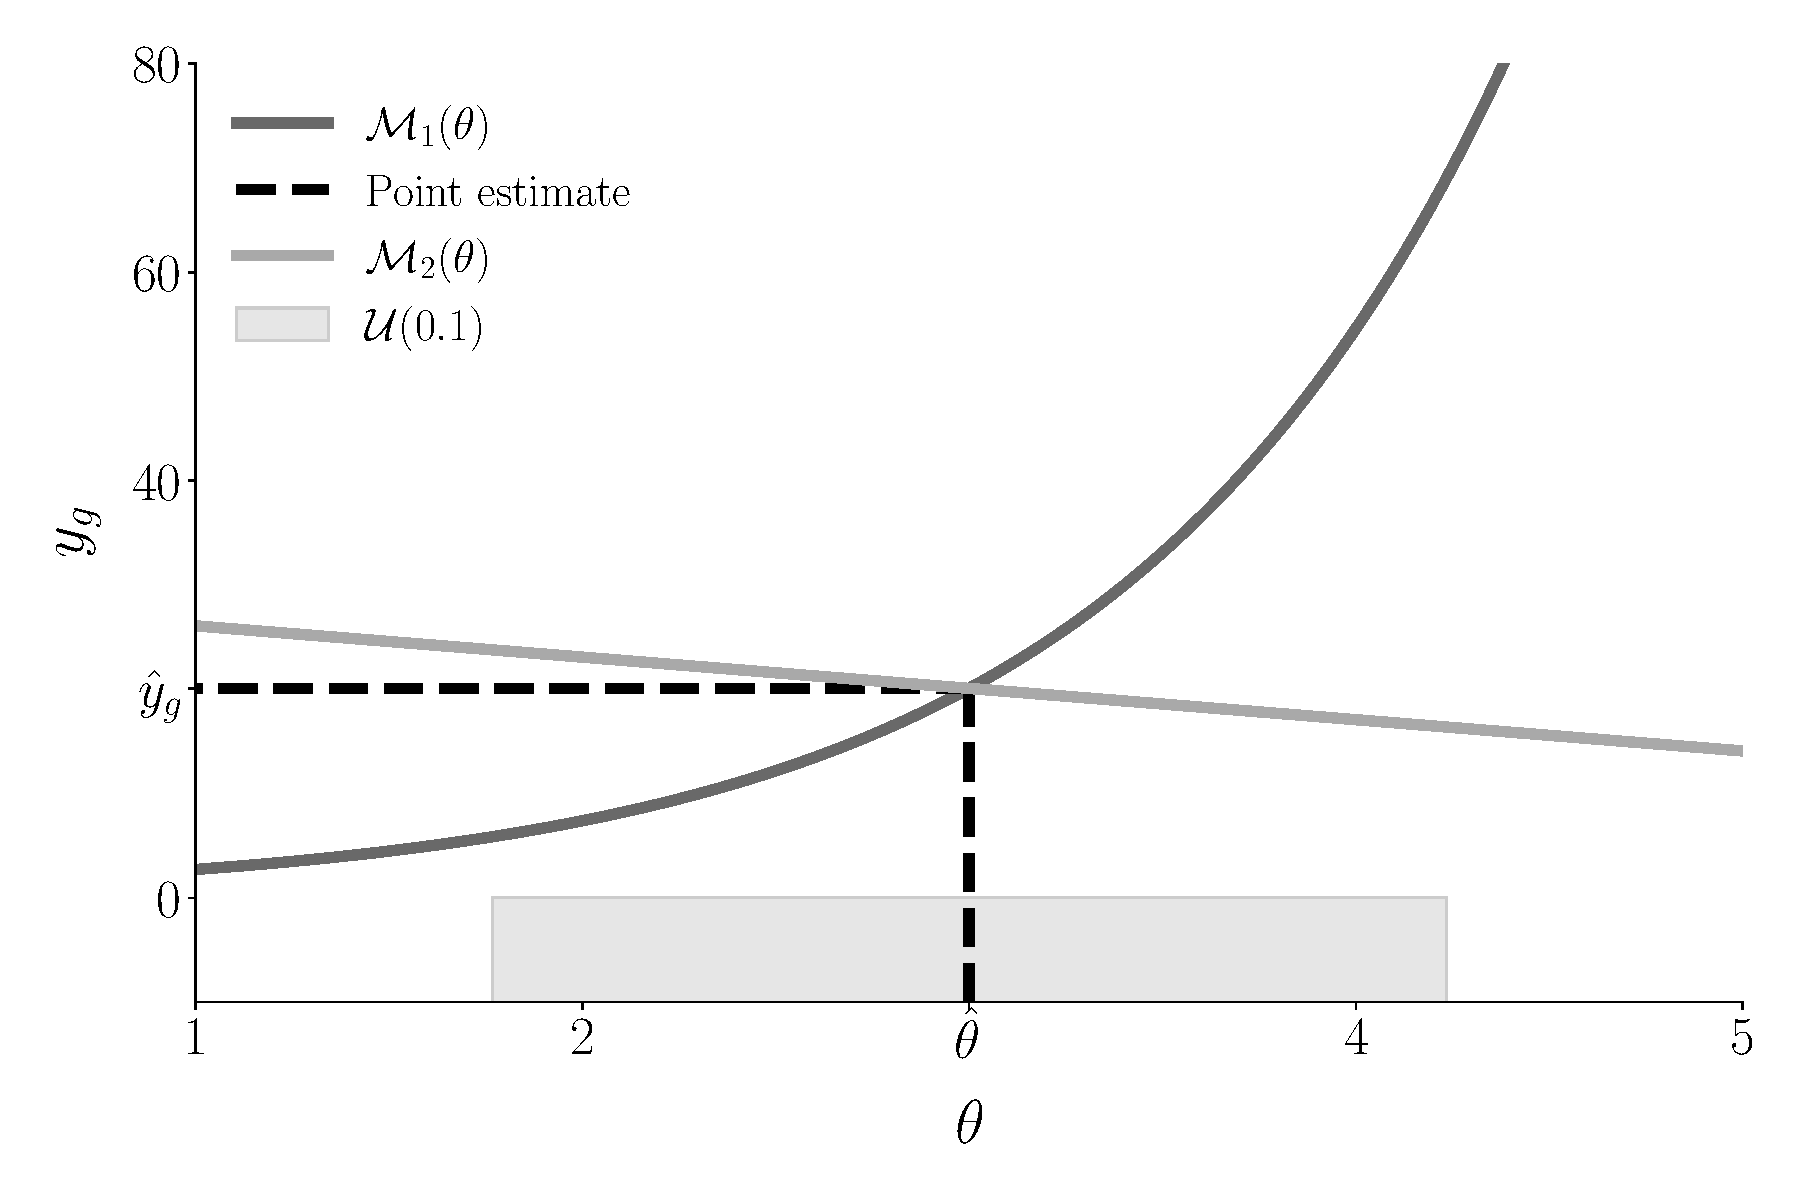
\includegraphics{fig-illustration-comparison-model-4-bw}}
\caption{Model comparison}\label{Illustration model comparison}
\begin{center}
\begin{minipage}[t]{0.6\columnwidth}
\item \scriptsize{\textbf{Notes:} We parameterize the two models as $y_1  = \exp{\theta}$ and $y_2 = 29.08 -3\, \theta$.}
\end{minipage}\end{center}
\end{figure}\FloatBarrier
%
\noindent Figure \ref{Illustration model comparison} traces the counterfactual from both models over a range of the parameter. At the point estimate, both models yield the same value for the counterfactual. Once we account for uncertainty in our estimates of the true parameter, deciding which policy to adopt becomes less straightforward: for higher values of $\theta$, the first policy is preferred, while the opposite is true for lower values.%---------------------------------------------------------------------------------------------------
%---------------------------------------------------------------------------------------------------
\subsection{Uncertainty sets}\label{Uncertainty set}
%---------------------------------------------------------------------------------------------------
%---------------------------------------------------------------------------------------------------
\citet{Manski.2021} suggests acknowledging parametric uncertainty by working with estimated confidence sets instead of point estimates. A confidence set $\bTheta(\alpha) \subset \bTheta$ covers the true parameters, from an ex-ante point of view, with a predetermined coverage probability of $(1 - \alpha)$. Proceeding with our analysis, we refine the status quo procedure, in which estimated parameter values serve as a stand-in for the model's true parametrization. Instead, we assume the estimated confidence set for the parameters  $\hat{\bTheta}(\alpha)$ and the counterfactual $\hat{\bTheta}_{y_g}(\alpha)$ are correct and analyze policy decisions accordingly. \\

\noindent Based on the estimated confidence sets, we construct so-called uncertainty sets for the parameters $\U(\alpha)$ and the prediction $\U_{y_g}(\alpha)$ by only considering parameterizations that we cannot reject based on a hypothesis test with confidence level $1 - \alpha$. This approach ensures the tractability of our decision-theoretic analysis, as the uncertainty set of the parameters is much smaller than the whole parameter space of the model. We adopt this procedure from the literature on data-driven robust optimization in operations research \citep{Ben-Tal.2013,Bertsimas.2018}.
%---------------------------------------------------------------------------------------------------
%---------------------------------------------------------------------------------------------------
\subsection{Statistical decision theory}\label{Statistical decision theory}
%---------------------------------------------------------------------------------------------------
%---------------------------------------------------------------------------------------------------
\noindent In our setting, a policy-maker relies on a structural model with an uncertain parametrization to map alternative policies to counterfactual predictions. In most cases, the preferred policy depends on the model's uncertain true parameters. We, therefore, draw on statistical decision theory to organize the decision-making process \citep{Gilboa.2009,Marinacci.2015}.\\

\noindent Returning to our example, we rank the two policies according to alternative statistical decision rules using an uncertainty set derived from a confidence set with a $90\%$ coverage probability. In what follows, we postulate a simple linear utility function $U(y_g)$ to describe the policy-maker's preferences.\footnote{We assume that the sampling distribution of the point estimate is normal with a mean of three and a standard deviation of three-fourths. We can derive the uncertainty sets directly and simply consider realizations of $\theta\in[1.76, 4.23]$.}\\

\noindent Figure \ref{Comparing policy predictions} shows the implied sampling distribution of the predictions for the two alternative policies and the corresponding uncertainty sets $\U_{y_g}(0.1)$. The mapping $\M_1$ is highly nonlinear, while the mapping $\M_{2}$ is linear. When evaluated at the point estimate, the counterfactual is the same under both policies, so a policy-maker is indifferent. However, the spread of the uncertainty set differs considerably.\\

\begin{figure}[h!]\centering
\scalebox{0.35}{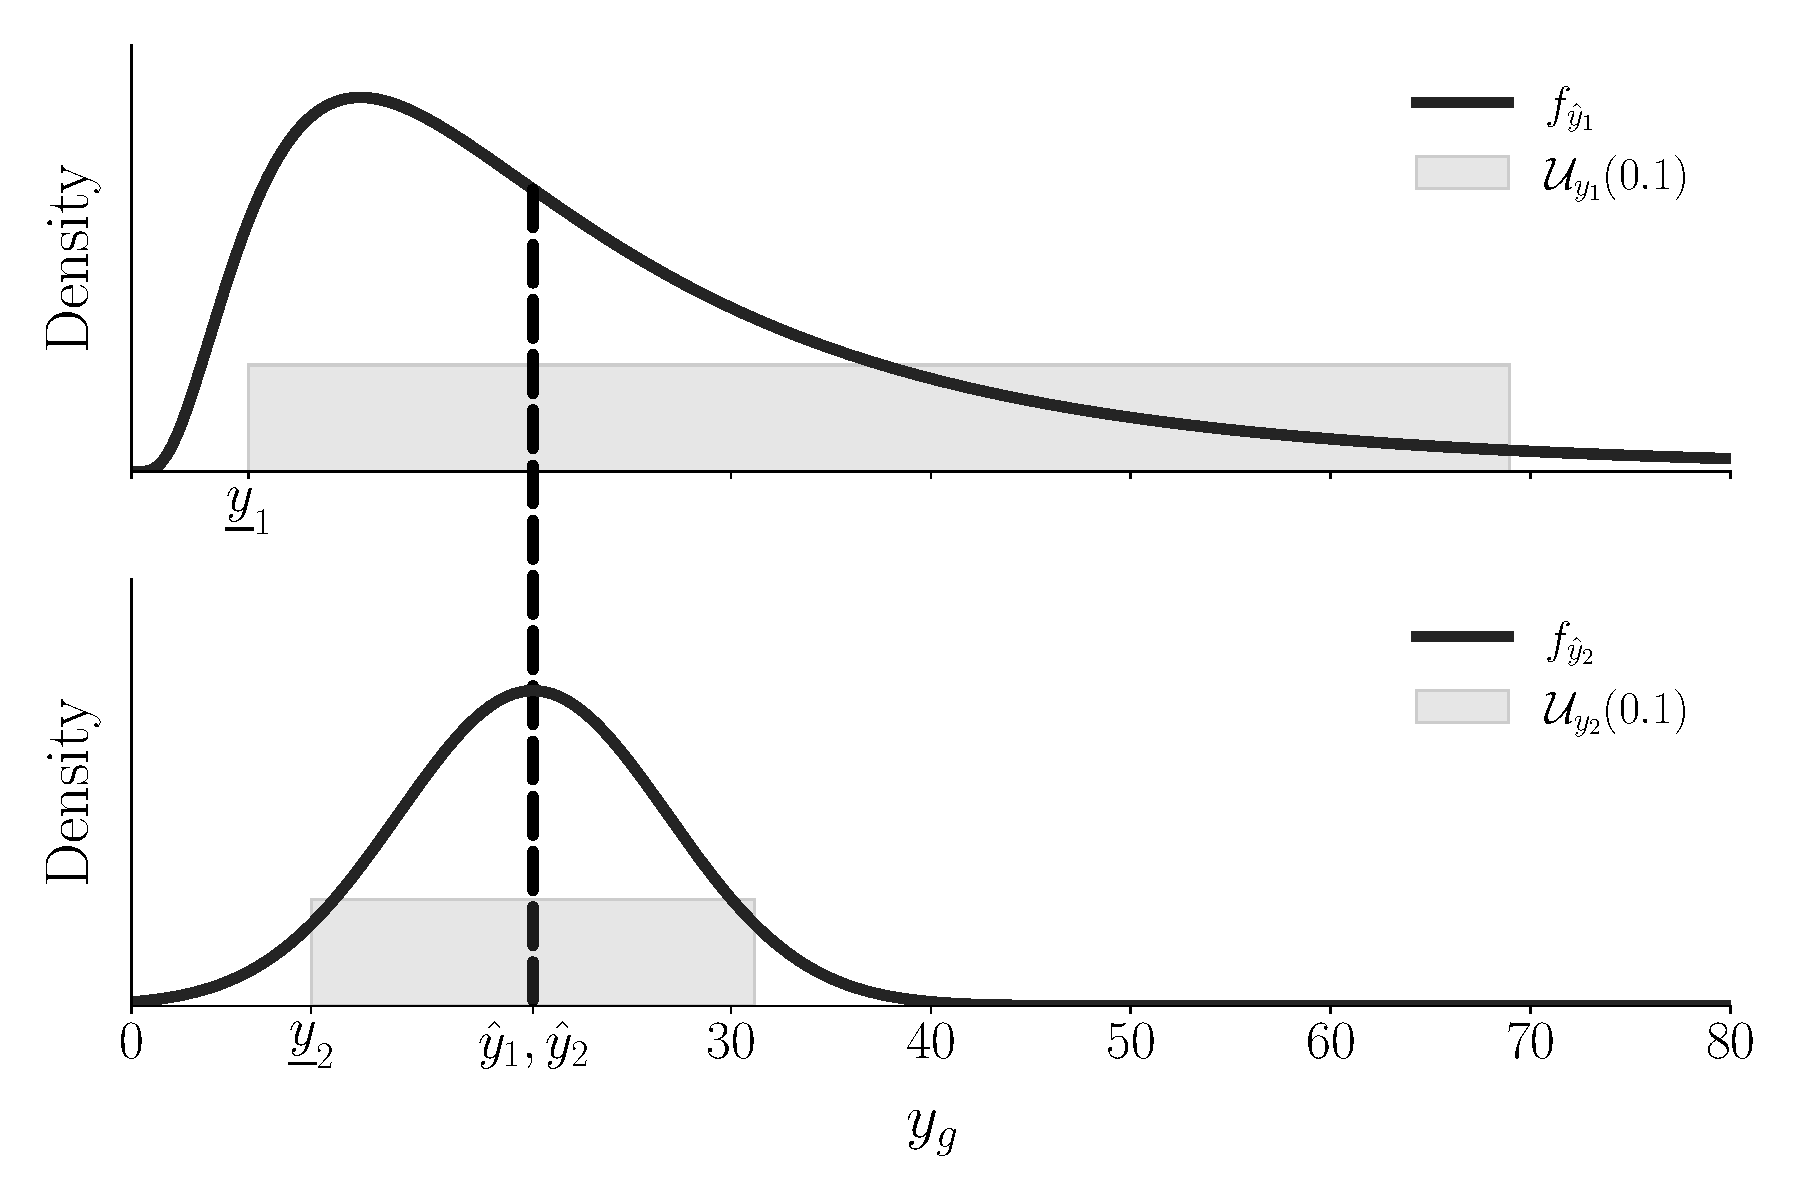
\includegraphics{fig-illustration-comparison-bw}}
\caption{Comparing policy predictions}\label{Comparing policy predictions}
\end{figure}\FloatBarrier

\noindent Decision theory proposes a variety of different rules for reasonable decisions in this setting. We explore the following four: (1) as-if optimization, (2) maximin criterion, (3) minimax regret rule, and (4) subjective Bayes.\\

\noindent As-if optimization describes the predominant practice. The estimation of the model produces point estimates that serve as a plug-in for the true parameters. The decision maximizes the utility at the point estimate. More formally,
%
\begin{align*}
  g^* =\argmax_{g \in \G} U(M_g(\hat{\btheta})).
\end{align*}
%
Given our example, an as-if policy-maker is indifferent between the two policies, since both policies result in the same counterfactual at the point estimates as indicated by the dashed line in Figure \ref{Comparing policy predictions}.\\

\noindent The maximin criterion and minimax regret rule are two common alternatives that favor actions that work uniformly well over all possible parameters in the uncertainty set. This approach departs from as-if optimization, which only considers a policy's performance at a single point in the uncertainty set. The maximin decision \citep{Gilboa.1989, Wald.1950} is determined by computing the minimum utility for each policy within the uncertainty set and choosing the one with the highest worst-case outcome. Stated concisely,
%
\begin{align*}
 g^* =\argmax_{g \in \G}\min_{\btheta \in \U(\alpha)} U(M_g(\btheta)).
\end{align*}
%
\noindent Returning to Figure \ref{Comparing policy predictions}, a maximin policy-maker prefers $g_2$ as the worst-case outcome. Within the uncertainty set, $\underline{y}_2$ is better than under the alternative policy, $g_1$.\\

\noindent The minimax regret rule \citep{Manski.2004, Niehans.1948} computes the maximum regret for each policy over the whole uncertainty set and chooses the policy that minimizes the maximum regret. The regret of choosing a policy $g$ for a given parameterization of the model is the difference between the maximum possible utility achieved from adopting $\tilde{g} \in \G$ and the actual utility obtained. The decision maximizes:
%
\begin{align*}
  g^* =\argmin_{g \in \G} \max_{\btheta \in \U(\alpha)}  \underbrace{\left[\max_{\tilde{g} \in \G} U(M_{\tilde{g}}(\btheta)) - U(M_g(\btheta)) \right]}_{\text{regret}}.
\end{align*}
%
\noindent Figure \ref{Comparing policy regret} compares our two policy examples over the uncertainty sets. A policy-maker adopting policy $g_1$ regrets his choice for small values of the model parameter, while the opposite is true for larger values. The regret of each policy is maximized at the boundaries of the uncertainty set. Maximum regret is minimized when a policy-maker chooses $g_1$. It corresponds to the difference in the counterfactual at the lower boundary of the uncertainty set instead of the larger difference at its upper bound. This outcome contradicts the maximin decision in which policy $g_2$ is preferred.

\begin{figure}[h!]\centering
\scalebox{0.35}{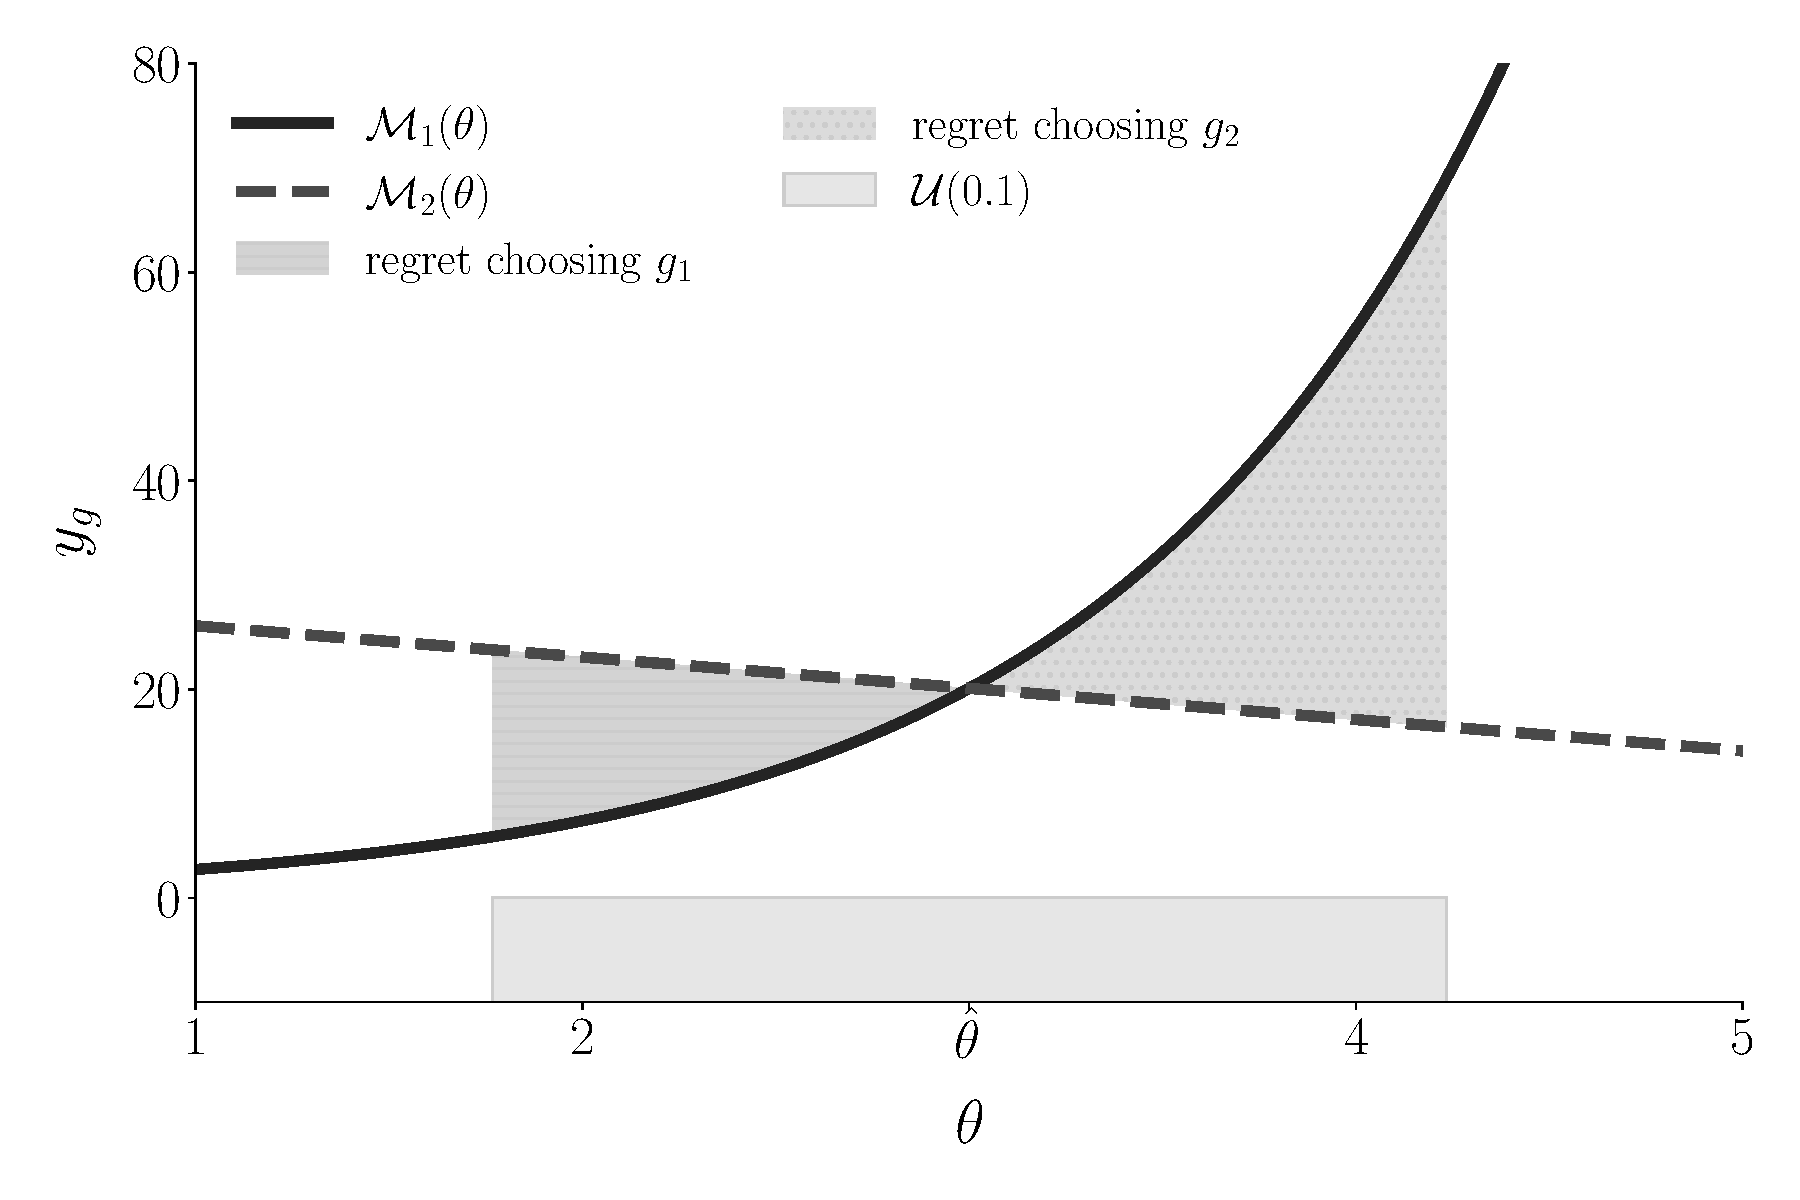
\includegraphics{fig-illustration-comparison-regret-bw.pdf}}
\caption{Comparing policy regret}\label{Comparing policy regret}\vspace{0.5cm}
\end{figure}\FloatBarrier

\noindent Each decision rule presented so far focuses on a single point in the uncertainty set as the policy's relevant performance measure. Bayesian approaches aggregate a policy's performance over the complete uncertainty set.\\

\noindent Maximization of the subjective expected utility \citep{Savage.1954} requires the policy-maker to place a subjective probability distribution $f_{\btheta}$ over the parameters in the uncertainty set.  A policy-maker then selects the alternative with the highest expected subjective utility. Formally,
%
\begin{align*}
  g^* =\argmax_{g \in \G} \int_{\U(\alpha)} U(M_g({\btheta})) \diff f_{\btheta}.
\end{align*}
%
\noindent Applying a uniform distribution to our example, a policy-maker chooses $g_1$, which performs well for high values of $\btheta$ and still reasonably well for low values.
